\documentclass[pdf]{beamer}
\setbeamertemplate{frametitle continuation}{\gdef\beamer@frametitle{}}
\usetheme{Madrid}
\definecolor{orange}{RGB}{242, 151, 36}
\setbeamercolor{palette primary}{bg=orange,fg=black}
\setbeamercolor{palette secondary}{bg=orange,fg=black}
\setbeamercolor{palette tertiary}{bg=orange,fg=black}
\setbeamercolor{palette quaternary}{bg=orange,fg=black}
\setbeamercolor{structure}{fg=orange}
\setbeamercolor{section in toc}{fg=orange}
\usepackage[utf8]{inputenc}
\usepackage[T1]{fontenc}
\usepackage{graphicx}
\graphicspath{ {images/} }



\title[Grafička sučelja u Gitu]
{Grafička sučelja u Gitu}
 
\author[Buterin, Dizdarević, Petrović]
{Ivan Buterin, Damir Dizdarević, Ana Petrović}
 
\institute[]
{
  Tehnički fakultet Sveučilišta u Rijeci\\
  Preddiplomski studij računarstva
}
 
\date[23.siječnja 2018.]
 
\begin{document}
\frame{\titlepage}
\frame{\frametitle{Sadržaj}
\tableofcontents[]}
\section{Uvod}
\begin{frame}[allowframebreaks]
\frametitle{Uvod}
\begin{itemize}
\item Test1
\item Test2
\item Test3
\item Test1
\item Test2
\item Test3
\framebreak
\item Test1
\item Test2
\item Test3
\item Test1
\item Test2
\item Test3
\end{itemize}
\end{frame}
\section{Git Kraken}
\begin{frame}[allowframebreaks]
\frametitle{Git Kraken}

\begin{itemize}
 \item dostupan za uporabu na Windows, Linux i Mac os operacijskim sustavima


 \item \textbf{Namjena:} 
 \item osnažiti produktivnost Git korisnika kroz \textbf{značajke} kao što su:
  {\setlength\itemindent{15pt}\item vizualna interakcija i savjeti}
  {\setlength\itemindent{15pt}\item samostalnost, učinkovitost, pouzdanost}
  {\setlength\itemindent{15pt}\item podržavanje više profila}
  {\setlength\itemindent{15pt}\item podržavanje funkcije poništavanja i ponovnog odabira jednim klikom}
  {\setlength\itemindent{15pt}\item ugrađeni alat za spajanje}
  {\setlength\itemindent{15pt}\item brz i intuitivan alat za pretraživanje}
  {\setlength\itemindent{15pt}\item prilagodljivost korisničkom radnom prostoru}
  {\setlength\itemindent{15pt}\item podržava i submodule i Gitflow}
  {\setlength\itemindent{15pt}\item integrira se s korisnikovim GitHub ili Bitbucket računom}
  {\setlength\itemindent{15pt}\item tipkovnički prečaci...}
 \framebreak
 \item radi sve standardne stvari koje bi trebali učiniti s git klijentom:
 		\item \textit{grananje}
 		\item \textit{spajanje}
 		\item \textit{povlačenje}
 		\item \textit{guranje}
 		\item \textit{vraćanje}
\framebreak
\item koristan za vizualizaciju prošlih radova

\end{itemize}

\begin{center}
    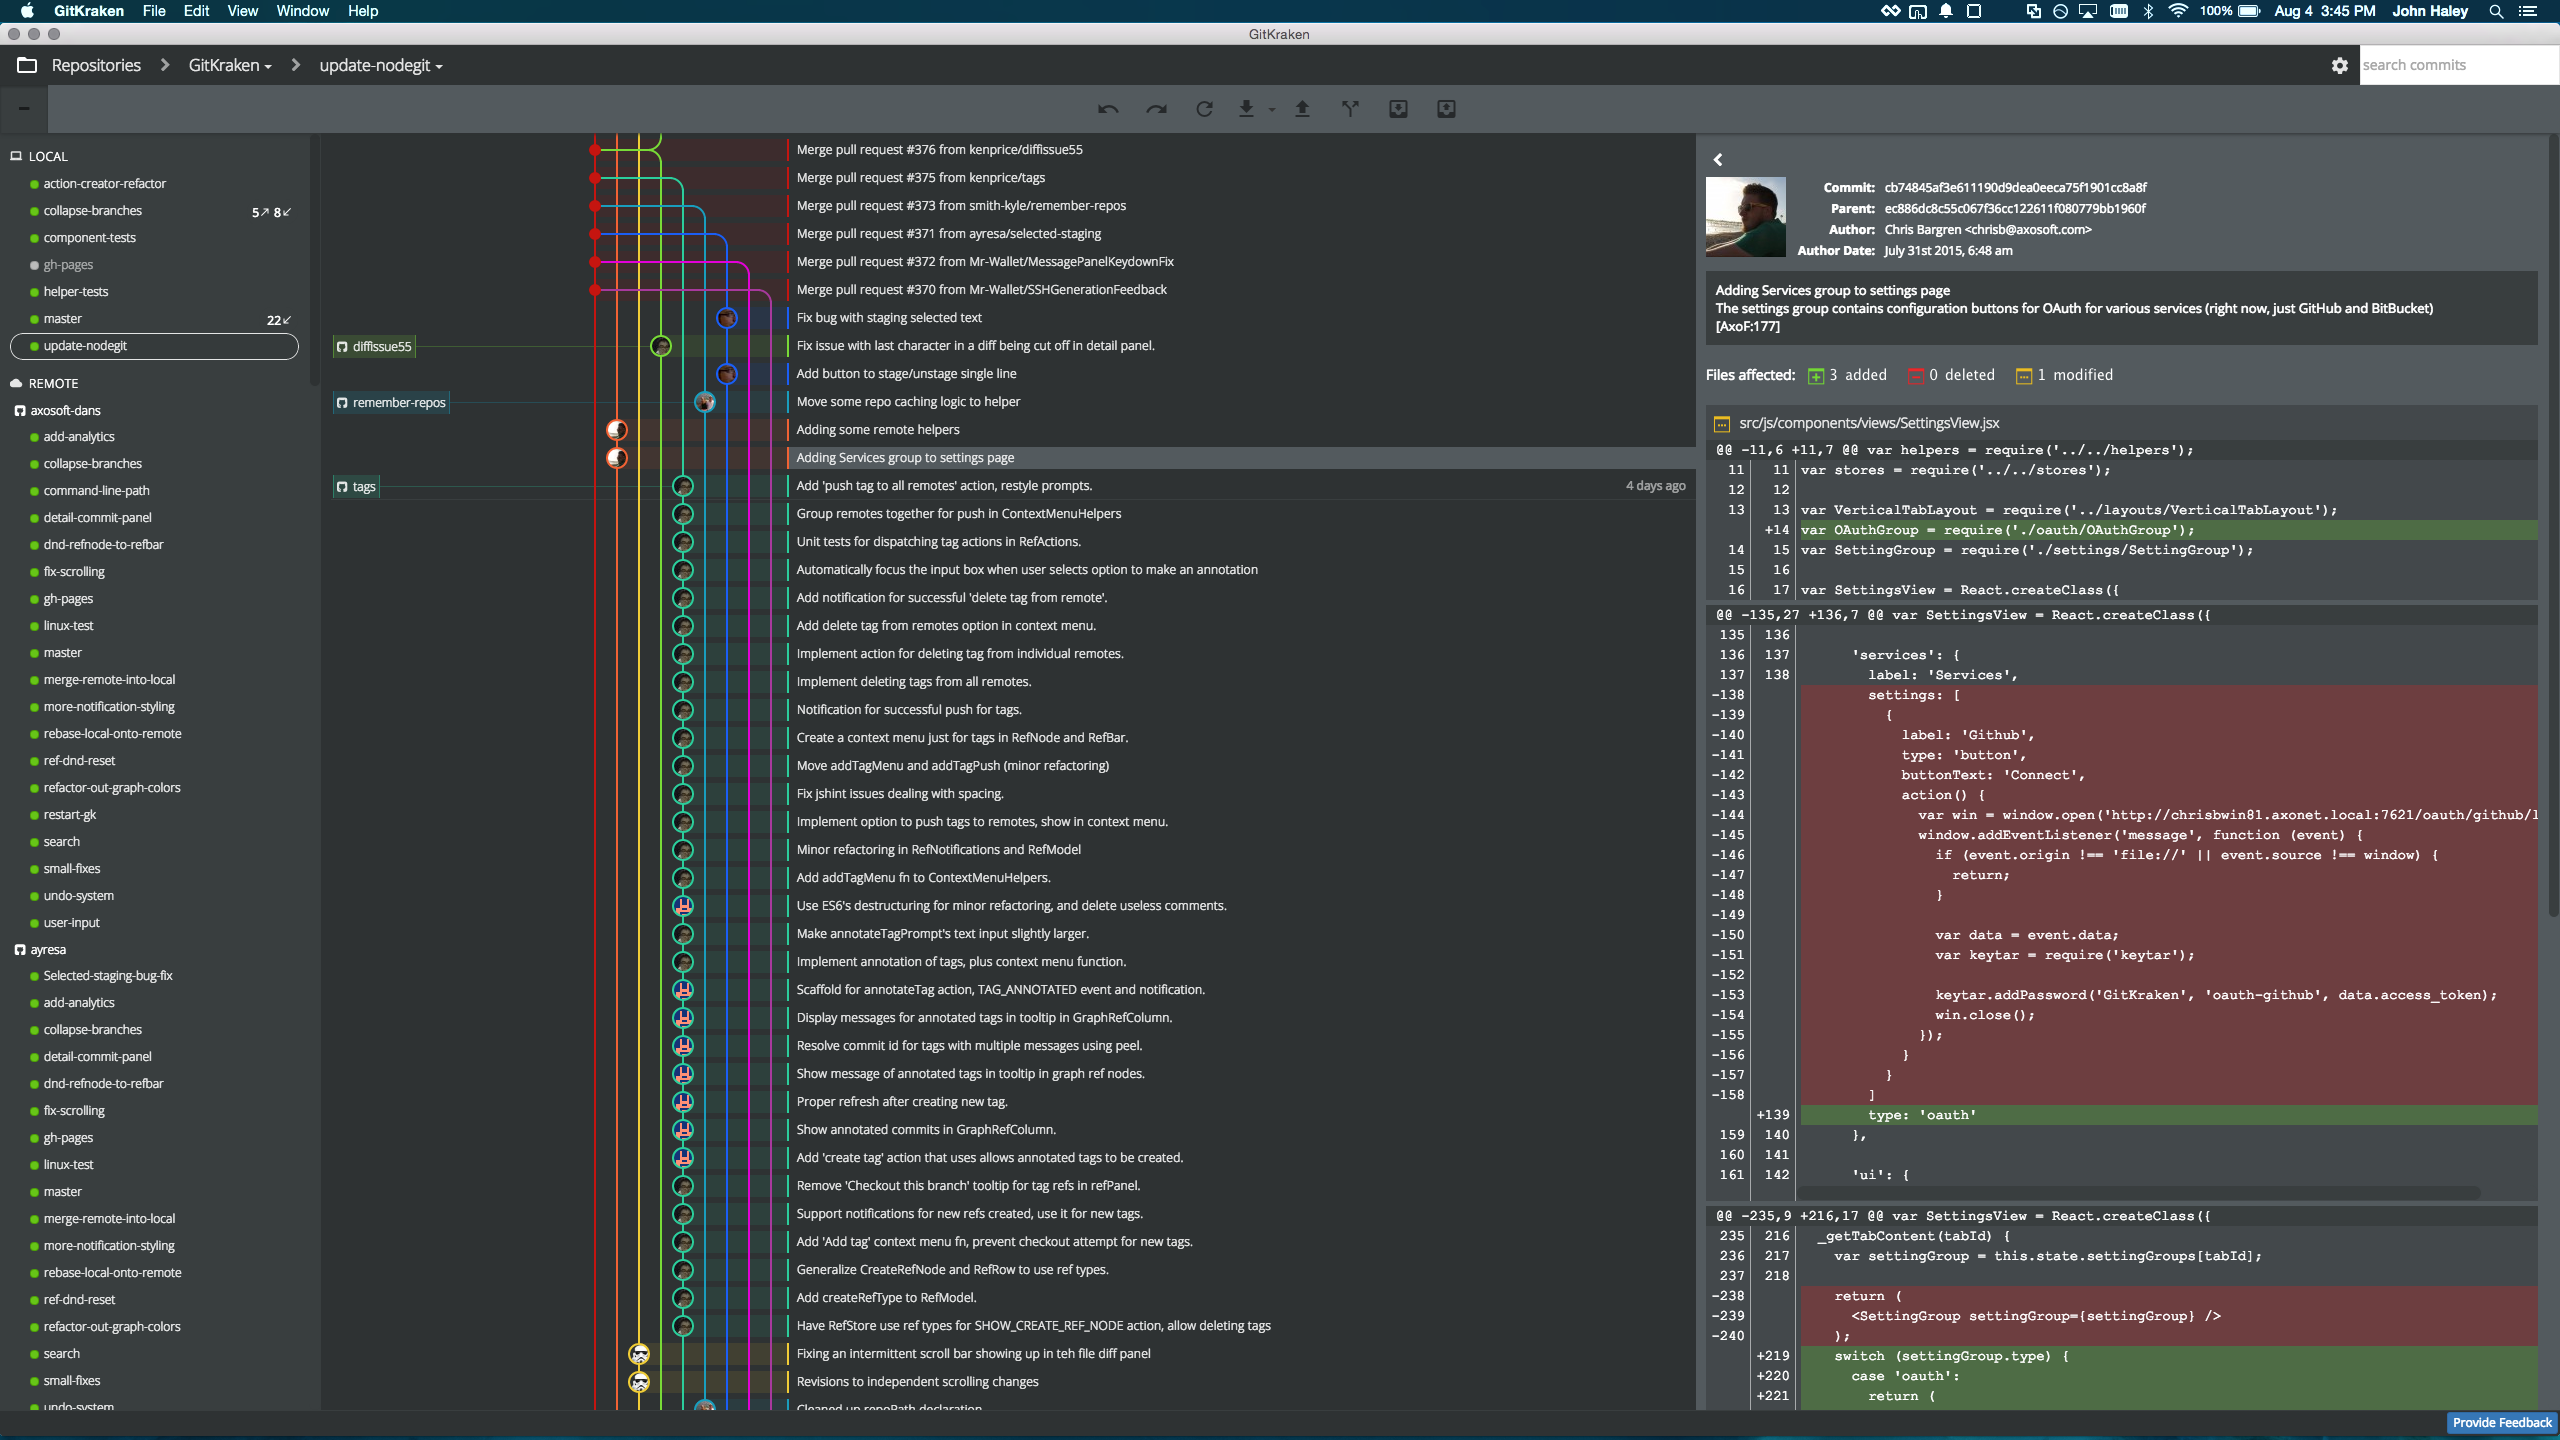
\includegraphics[width=0.8\linewidth]{images/gitkraken-UI.png}
\end{center}

\end{frame}
\section{Git Tortoise}
\begin{frame}[allowframebreaks]
\frametitle{Git Tortoise}
\begin{itemize}
\item Jednostavan za korištenje:
\item sve naredbe dostupne su izravno iz Windows Explorera 
\item pregled statusa datoteka izravno u programu Windows Exploreru
\item opisni dijalozi, stalno se poboljšava zbog povratnih informacija korisnika
\item dopušta premještanje datoteka
\framebreak
\item kontekstni izbornik je glavni način interakcije s TortoiseGit
 \item Na sljedećoj slici vidite nekoliko mogućih opcija: 
 \framebreak
 \item Snažan dijaloški okvir za izvršavanje 
 \item provjeru pravopisa za dnevničke poruke
 \item automatsko dovršavanje putova i ključnih riječi modificiranih datoteka
 \item oblikovanje teksta s posebnim oznakama
 \framebreak
 \item  Integracija s sustavima za praćenje problema
 \item pruža fleksibilan mehanizam za integraciju bilo kojeg web sustava za praćenje bugova
 \item zaseban ulazni okvir za unos broja izdanja dodijeljenog obvezi ili bojanje broja izdavanja izravno u samoj zaporci
 \item kada se prikaže sve dnevničke poruke, dodaje se dodatni stupac s brojem izdavanja (odmah možete vidjeti kome se pripisuje obveza)
 \item brojevi izdanja pretvaraju se u veze koje otvaraju webbrowser izravno na odgovarajućem broju
 \item opcionalno upozorenje ako se obveza ne dodjeljuje broju izdavanja
 \framebreak
 \item Korisni alati
 \item tortoiseGitMerge 
 \item prikazuje promjene koje ste napravili u datotekama
 \item pomaže u rješavanju sukoba
 \item može primijeniti patchfile koje ste dobili od korisnika bez predajnog pristupa vašem spremištu
 \item TortoiseGitBlame: prikazati krivnju datoteka
 \item prikazuje i zapisničke poruke za svaku liniju u datoteci
 \item TortoiseGitIDiff: da biste vidjeli promjene koje ste napravili na slikovnim datotekama 
 \framebreak
 \item Dostupno na mnogim jezicima
 \item TortoiseGit je stabilan
 \item tortoiseGit je klijent za kontrolu revizije Git
 \item besplatni je softver objavljen pod GNU General Public License.
 \item u programu Windows Explorer, osim prikazivanja stavki izbornika u kontekstu za Git naredbe
 \item tortoiseGit nudi ikonske slojeve koji upućuju na status Gitovih stabala i datoteka.
 \item također dolazi s TortoiseGitMerge programom za vizualno usporedbu dviju datoteka i rješavanje sukoba.
\end{itemize}
\end{frame}
\section{SmartGit}
\begin{frame}[allowframebreaks]
\frametitle{SmartGit}
 
\begin{itemize}
 \item podržan od strane svih operacijskih sustava
 \item najpogodniji za timski rad na velikim projektima
 \item nesmetan rad na aktivnom projektu
 \item podržan i na drugim Git, kao i SVN platformama
 \item podržava Markdown
 \item jedan od najboljih uslužnih programa za usporedbu datoteka koji jasno predočava promjena napravljene kroz povijest
 \framebreak
 \item na tržistu od 2009. godine
 \item najpogodniji za početnike
 \item integrira s GitHubom, BitBucketom i GitLabom
\end{itemize}

\begin{figure}[h]
	\centering
	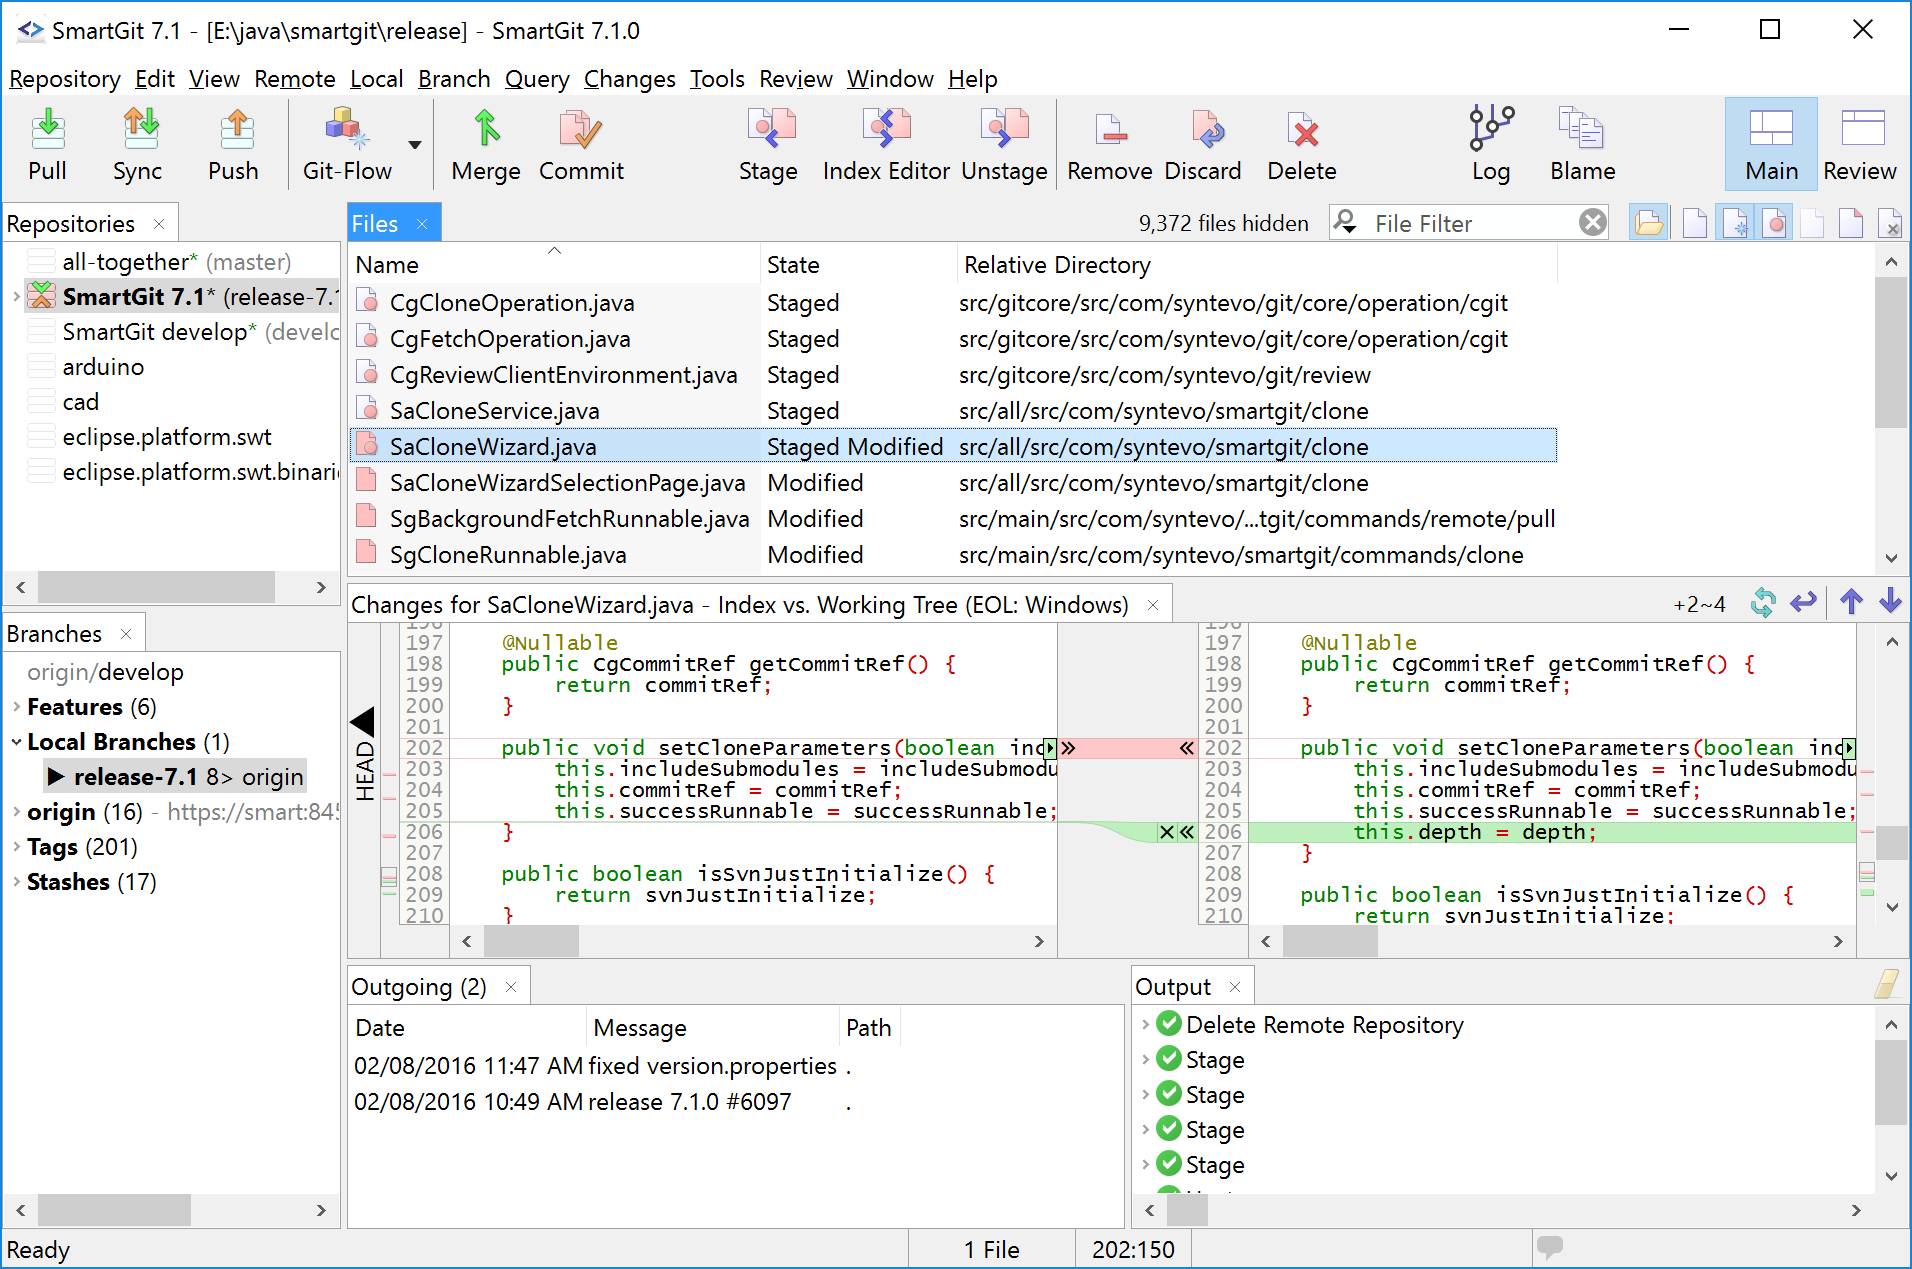
\includegraphics[width=0.9\linewidth]{images/git-project.png}
\end{figure}
\end{frame}

\input{git_extensions.tex}
\section{GitEye}
\begin{frame}[allowframebreaks]
\frametitle{GitEye}
 
\begin{itemize}
 \item koristan za velike kompanije - lakoćom se upravlja važnim projektima
 \item povlači repozitorije gdje god se oni nalazili
 \item poseban modul praćenja promjena datoteka - više ljudi radi na dokumentu bez da smetaju jedno drugome
 \item integrira se s uslugama razvojnih programera treće strane kako bi se olakšao proces upravljanja projektima
 \framebreak
 \item korisne i user-friendly značajke:
 		\item izvrsno sučelje
 		\item pristupačan pregled povijesti
 		\item besplatan i učestali update aplikacije
\end{itemize}


\end{frame}

\begin{figure}
	\includegraphics[width=0.9\linewidth]{images/giteye-git-client.jpg}
	\caption{GitEye sučelje}
\end{figure}

\input{gmaster.tex}
\input{gitahead.tex}
\section{Git Cola}
\begin{frame}[allowframebreaks]
\frametitle{Git Cola}
 
\begin{itemize}
 \item moćno grafičko sučelje za git
 \item besplatan software napisan u Pythonu
 \item podržava veliki broj tipkovničkih prečaca
 \item samostalan, učinkovit, pouzdan
 \item podesive varijable - promjena izgleda i ponašanja aplikacije
 \item aktivni životni ciklus razvoja s kontinuiranom optimizacijom značajki i funkcija
 \framebreak
 \item korisne i praktične značajke:
 		\item nadprosječno brz
 		\item besplatan za uporabu
 		\item ubrzanje komandnom linijom
 		\item mogućnosti konfiguriranja za prijavu
\end{itemize}


\begin{figure}
	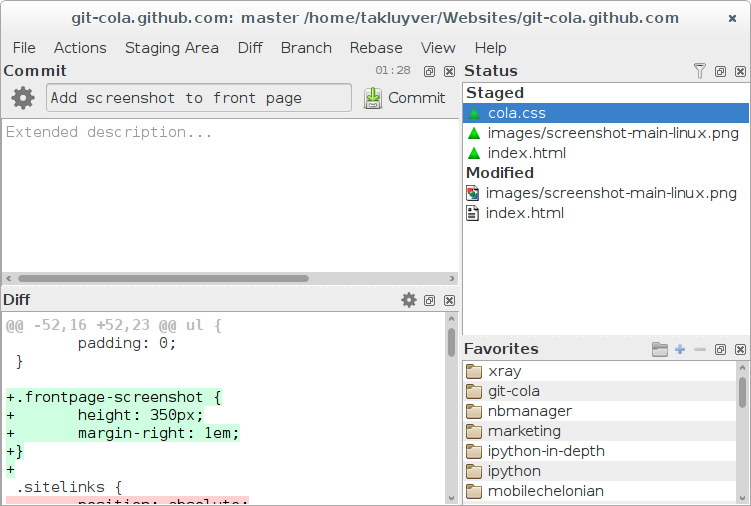
\includegraphics[width=0.9\linewidth]{images/git-cola.png}
\end{figure}
\end{frame}

\input{giggle.tex}
\input{gitg.tex}
\input{ogit.tex}
\input{gitforce.tex}
\input{egit.tex}
\end{document}
